\documentclass[journal]{vgtc}                % final (journal style)
%\documentclass[review,journal]{vgtc}         % review (journal style)
%\documentclass[widereview]{vgtc}             % wide-spaced review
%\documentclass[preprint,journal]{vgtc}       % preprint (journal style)
%\documentclass[electronic,journal]{vgtc}     % electronic version, journal

%% Please use one of the ``review'' options in combination with the
%% assigned online id (see below) ONLY if your paper uses a double blind
%% review process. Some conferences, like IEEE Vis and InfoVis, have NOT
%% in the past.

\usepackage{mathptmx}
\usepackage{graphicx}
\usepackage{times}
\usepackage[usenames,dvipsnames,svgnames]{xcolor}
\usepackage[bookmarks,backref=true,linkcolor=black]{hyperref} 
\usepackage{subfigure}
\usepackage{gensymb}

\hypersetup{
  pdfauthor = {},
  pdftitle = {},
  pdfsubject = {},
  pdfkeywords = {},
  colorlinks=true,
  linkcolor= black,
  citecolor= black,
  pageanchor=true,
  urlcolor = black,
  plainpages = false,
  linktocpage
}

\onlineid{0}
\vgtccategory{Research}
\vgtcinsertpkg
%\preprinttext{To appear in IEEE Transactions on Visualization and Computer Graphics.}

\def\etal{\textit{et al.}}
\definecolor{MyGreen}{rgb}{0,0.7,0}
\definecolor{MyWhite}{rgb}{1,1,1}
\definecolor{MyGray}{rgb}{0.5,0.5,0.5}
\definecolor{LightGray}{rgb}{0.7,0.7,0.7}
\definecolor{DarkGray}{rgb}{0.3,0.3,0.3}
\definecolor{DarkYellow}{rgb}{0.7,0.7,0.0}
\definecolor{MyNavyBlue}{rgb}{0.2,0.3,0.7}
\definecolor{darkgreen}{rgb}{0,0.55,0}
\newcommand{\black}[1]{{\color{Black} #1}}
\newcommand{\white}[1]{{\color{MyWhite} #1}}
\newcommand{\gray}[1]{{\color{MyGray} #1}}
\newcommand{\red}[1]{{\color{red} #1}}
\newcommand{\green}[1]{{\color{MyGreen} #1}}
\newcommand{\blue}[1]{{\color{MyNavyBlue} #1}}
\newcommand{\yellow}[1]{{\color{DarkYellow} #1}}
\newcommand{\maybe}[1]{\yellow{#1}}
\newcommand{\rout}[1]{\red{\sout{#1}}}
\newcommand{\repl}[2]{\rout{#1} \green{#2}}
\newcommand{\fix}[1]{\red{\emph{(#1)}}}
\newcommand{\Fix}[1]{\begin{itemize} \renewcommand\labelitemi{\red{--}} \item \red{#1} \end{itemize}}

\newcommand{\todo}[1] {\textbf{[~}\textcolor {red}{#1}\marginpar{\textcolor {red}{\centerline{{\Huge \textbf{!}}}}}\textbf{~]}}
\newcommand{\question}[1] {\textbf{[~}\textcolor {darkgreen}{#1}\marginpar{\textcolor {darkgreen}{\centerline{{\Huge \textbf{!}}}}}\textbf{~]}}
\newcommand{\diff}[1]{[\textcolor{blue}{#1}\marginpar{\textcolor{blue}{\centerline{{\Huge \textbf{!}}}}}]}

\title{Visual Verification of Space Weather Ensemble Simulations}

\author{
%    Alexander~Bock,~\textit{Student Member,~IEEE,}
    Alexander~Bock,
    Asher Pembroke,
    M. Leila Mays,
    Lutz Rastaetter,\\%
%    Anders Ynnerman,~\textit{Member, IEEE,}
    Anders Ynnerman,
%    and Timo Ropinski~\textit{Member, IEEE}%
    and Timo Ropinski%
}

\authorfooter {
  \item A. Bock, A. Ynnerman are with Scientific Visualization Group, Link\"oping University, Sweden. E-mail: \{alexander.bock\,$\vert$\,anders.ynnerman\}@liu.se.
  \item A. Pembroke, ML Mays, and L. Rastaetter are with NASA Goddard Space Flight Center, Greenbelt, Maryland. E-mail: \{asher.d.pembroke\,$\vert$\, m.leila.mays\,$\vert$\, lutz.rastaetter\}@nasa.gov.
  \item T. Ropinski is with the Visual Computing Group, Ulm University. E-mail: timo.ropinski@uni-ulm.de.
}

\shortauthortitle{Bock \MakeLowercase{\textit{et al.}}: Visual Verification of Space Weather Simulations}

%% Abstract section.
\abstract{%
Supporting the growing field of space weather forecasting, we propose a system to analyze and contextualize simulations of coronal mass ejections. As the current simulation techniques require manual input, uncertainty is introduced into the simulation pipeline leading to inaccurate predictions that can be mitigated by using ensemble simulations. In our system, we provide the space weather analyst with a multi-view system that provides visualizations to: 1. compare ensemble members against in-situ ground truth data (arrival time and geoeffectivity), 2. inspect time-dependent information derived from optical flow analysis of satellite imagery, and 3. combining images from multiple satellites with a volumetric rendering of magnetohydrodynamics simulations. This three-tier workflow provides the experts with the tools to increase knowledge about not yet fully understood principles underpinning the evolution and propagation of coronal mass ejections which pose a danger to Earth and interplanetary travel.

% Including more visualization in the end
% Added sentences for the different views
% 

%The current workflow requires the manual selection of parameters which introduces uncertainy into the simulation pipeline, leading to inaccurate predictions. We present a system that combines satellite imagery from the SOHO, STEREO A, and STEREO B satellites with a volumetric rendering of magnetohydrodynamics simulations of the solar system in order to provide space weather analysts with the means to compare ensemble runs against the ground truth data, thus fostering knowledge about space weather phenomena. Comparisons are performed on static information such as arrival time and time-varying information retrieved by extracting the optical flow from the satellite images and comparing that to the simulated velocity. The system provides a novel technique to simultaneously inspect the time-dependent quality measures of all observation instruments (SOHO [LASCO C3], STEREO A and B [Cor2, HI 1, and HI 2]) and allow the analyst to make an informed decision about the accuracy of the simulation.

%The current technique of simulating coronal mass ejections in ENLIL simulations requires cone parameters that are manually derived from STEREO satellite imagery. This manual input is not perfect and introduces uncertainty into the simulation pipeline, leading to inaccurate predictions. We present a system that embeds satellite imagery from SOHO and STEREO A and B into a 3D volumetric rendering of ENLIL simulations. By extracting the optical flow from the images and renderings, we retrieve pairs of velocity fields that are utilized to derive a quality measure that is used to test the simulation against the ground truth satellite image data. The system provides a novel technique to simultaneously inspect the time-dependent quality measures of all observation instruments (SOHO [LASCO C3], STEREO A and B [Cor2, HI 1, and HI 2]) and allow the analyst to make an informed decision about the accuracy of the simulation. Lastly, we extend this system to deal with ensemble runs, generated by varying the cone parameters. The aforementioned quality measures are generated for each ensemble member and the system provides an interface to browser and assess the whole ensemble run at once, enabling the analyst to quickly select the ensemble member agreeing with the satellite data.%
} % end of abstract

%% Keywords that describe your work. Will show as 'Index Terms' in journal
%% please capitalize first letter and insert punctuation after last keyword
\keywords{Visual Verification, Space Weather, Coronal Mass Ejections, Ensemble}

%% ACM Computing Classification System (CCS). 
%% See <http://www.acm.org/class/1998/> for details.
%% The ``\CCScat'' command takes four arguments.

\CCScatlist{ % not used in journal version
 \CCScat{K.6.1}{Management of Computing and Information Systems}%
{Project and People Management}{Life Cycle};
 \CCScat{K.7.m}{The Computing Profession}{Miscellaneous}{Ethics}
}

%% Uncomment below to include a teaser figure.
\teaser{
  \newcommand{\abImageHeight}{3.25cm}
  \centering
  
  \subfigure[Ensemble Selection View] {
    \fbox{\includegraphics[height=\abImageHeight]{figures/EnsembleSelectionView.png}}
  }
  \subfigure[Timeline View] {
    \fbox{\includegraphics[height=\abImageHeight]{figures/TimelineView.png}}
  }
  \subfigure[Rendering View] {
    \fbox{\includegraphics[height=\abImageHeight]{figures/RenderingView.png}}
  }
  \caption{The three different views our proposed system uses to help space weather analysts gaining a better understanding of ensemble simulations of coronal mass ejections. The Ensemble Selection View (a) provides comparisons with ground-truth, in-situ measurements. The Timeline View (b) enables the comparison of time-dependent data derived from satellite images. The Rendering View (c) allows the inspection of all data in a single scene.}
  \label{fig:teaser}
}

%% Uncomment below to disable the manuscript note
%\renewcommand{\manuscriptnotetxt}{}

%% Copyright space is enabled by default as required by guidelines.
%% It is disabled by the 'review' option or via the following command:
% \nocopyrightspace

\def\etal{\textit{et al.}}
%\renewcommand\floatpagefraction{1.0}
%\renewcommand\topfraction{1.0}
%\renewcommand\bottomfraction{.9}
%\renewcommand\textfraction{.1}
%\setcounter{totalnumber}{20}
%\setcounter{topnumber}{10}
%\setcounter{bottomnumber}{10}
\definecolor{MyGreen}{rgb}{0,0.7,0}
\definecolor{MyWhite}{rgb}{1,1,1}
\definecolor{MyGray}{rgb}{0.5,0.5,0.5}
\definecolor{LightGray}{rgb}{0.7,0.7,0.7}
\definecolor{DarkGray}{rgb}{0.3,0.3,0.3}
\definecolor{DarkYellow}{rgb}{0.7,0.7,0.0}
\definecolor{MyNavyBlue}{rgb}{0.2,0.3,0.7}
\definecolor{darkgreen}{rgb}{0,0.55,0}
\newcommand{\black}[1]{{\color{Black} #1}}
\newcommand{\white}[1]{{\color{MyWhite} #1}}
\newcommand{\gray}[1]{{\color{MyGray} #1}}
\newcommand{\red}[1]{{\color{red} #1}}
\newcommand{\green}[1]{{\color{MyGreen} #1}}
\newcommand{\blue}[1]{{\color{MyNavyBlue} #1}}
\newcommand{\yellow}[1]{{\color{DarkYellow} #1}}
\newcommand{\maybe}[1]{\yellow{#1}}
\newcommand{\rout}[1]{\red{\sout{#1}}}
\newcommand{\repl}[2]{\rout{#1} \green{#2}}
\newcommand{\fix}[1]{\red{\emph{(#1)}}}
\newcommand{\Fix}[1]{\begin{itemize} \renewcommand\labelitemi{\red{--}} \item \red{#1} 
\end{itemize}}

\newcommand{\todo}[1] {\textbf{[~}\textcolor {red}{#1}\marginpar{\textcolor {red}{\centerline{{\Huge \textbf{!}}}}}\textbf{~]}}
\newcommand{\question}[1] {\textbf{[~}\textcolor {darkgreen}{#1}\marginpar{\textcolor {darkgreen}{\centerline{{\Huge \textbf{!}}}}}\textbf{~]}}
\newcommand{\diff}[1]{[\textcolor{blue}{#1}\marginpar{\textcolor{blue}{\centerline{{\Huge \textbf{!}}}}}]}

%%%%%%%%%%%%%%%%%%%%%%%%%%%%%%%%%%%%%%%%%%%%%%%%%%%%%%%%%%%%%%%%
%%%%%%%%%%%%%%%%%%%%%% START OF THE PAPER %%%%%%%%%%%%%%%%%%%%%%
%%%%%%%%%%%%%%%%%%%%%%%%%%%%%%%%%%%%%%%%%%%%%%%%%%%%%%%%%%%%%%%%%

\newcommand{\kpIndex}{$\textrm{K}_\textrm{P}$}
\setlength\fboxsep{0pt}

\begin{document}
\firstsection{Introduction}
\maketitle
%% \section{Introduction} %for journal use above \firstsection{..} instead
\emph{Space weather} is the description of the environmental conditions in our solar system and their effects on planets, spacecraft, and human society. The main factors in driving space weather in our solar system are created by the Sun. Coronal mass ejections (CMEs) occur when magnetic field lines on the Sun's surface reconnect and accelerate plasma clouds away from the Sun and into the solar system. \emph{Space weather forecasting} is, among others, the field of predicting the direction, velocity, and impact of CMEs when they hit objects in the solar system, like Earth or spacecraft. When spacecraft are hit by these events, they can cause irreparable damage to electronic systems. In the case of Earth, most of the plasma is deflected by Earth's magnetosphere and funneled towards the north and south pole, creating auroras. However, it also causes geomagnetically induced currents in terrestrial infrastructure, such as power grids. This happened in Quebec in 1989 when a CME struck Earth and induced currents in the power grid caused a blackout nine hours long. The biggest CME on record is the Carrington Event from 1859 that generated auroras as far south as the Sahara and induced currents in telegraph lines that gave electrical shocks to telegraph operators and sparked fires. An insurance agency estimated that, in North America alone, a similar event today would cause up to \$2.6 trillion in damages and create blackouts of up to 2 years due to destroyed transformers~\cite{lloyds2013impact}. However, that situation that can be completely mitigated by accurate space weather forecasting. In July of 2012 a Carrington-level CME occurred that almost hit Earth~\cite{baker2013major} and was not accurately predicted due to inaccuracies in the simulation process.

%ENLIL~\cite{odstrcil2003modeling} with the Wang-Sheeley-Arge model~\cite{parsons2011wang}, 
%The cone is used to generate an initial particle distribution for the simulation, which is then advected over time.
%While the ENLIL-WSA simulation is the state-of-the-art approach, the assumption of a conical shape of the CME is not true in general, further increasing the space weather analyst's need for a flexible verification tool.
Current CME predictions created by NASA and the National Oceanic and Atmospheric Administration are based on magnetohydrodynamic simulations whose input parameters are derived from satellite imagery. In the state-of-the-art simulation code, the CME is modeled as a cone originating from the Sun with a \emph{direction}, \emph{velocity}, and \emph{opening angle} as free parameters (see Figure~\ref{fig:enlil}). Currently, these cone parameters are manually derived from satellite images, which naturally introduces error into the simulation pipeline and thus requires verification. Providing a system to dealing with this uncertainty is the main contribution of this paper.

\begin{figure}
\newcommand{\abEnlilImageHeight}{0.45\columnwidth}
\centering
\subfigure[The ENLIL simulation with Cone parameters]{
  \fbox{\includegraphics[width=\abEnlilImageHeight]{figures/Enlil.jpg}}
    \label{fig:enlil}
  }
\hfill{}
\subfigure[Coronagraph image of a coronal mass ejection with the Earth for scale]{
  \fbox{\includegraphics[width=\abEnlilImageHeight]{figures/CME.png}}
  \label{fig:cme}
}
\caption{These images show the inputs of the simulation code ENLIL, that assumes a conical shape, described by four parameters, for a coronal mass ejection (a). (b) shows a coronal mass ejection with the Earth to scale.}
\end{figure}


To mitigate the impact of measurement inaccuracies, simulation ensembles are generated by varying the free parameters and performing simulations for each combination. A simulation run can be verified in two ways. One, if the CME impacts the Earth or any suitable spacecraft in the solar system, ground-truth in-situ measurements of the arrival time, velocity, and magnetic field strength are measured and compared against the values predicted by the simulation. Second, renderings of the simulation can be compared with imagery from spacecraft equipped with coronagraphs, a technique that is not currently in use at the space weather forecasting sites. Whereas the first comparison results in scalar values of the accuracy, image comparison can be performed for each available frame, thus producing time-varying information about the simulation's accuracy from multiple locations.

%Later:
%Currently, four spacecraft are capable of this technique; SDO is located on a geostationary orbit, SOHO is located at the L$_1$ point between Earth and the Sun, and STEREO A and STEREO B are on heliocentric orbits. STEREO A and B have three imagers ranging from the Sun's surface all the way to the orbit of Earth and provide a stereoscopic view of the interplanetary space between the Sun and the Earth~\ref{fig:spacecraftlocation}. As SDO and SOHO provide us with the same viewpoint towards the Sun and the SOHO is well-tested, we chose to discard the measurements from the SDO satellite.

Our proposed system provides the space weather analyst with a three step workflow utilizing a multi-view setup to quickly assess the quality and accuracy of all ensemble members. In the first step, the analyst compares all ensemble members at once to the acquired ground truth data in a glyph-based visualization provided access to the measured scalar values. This allows a quick reduction of the number of interesting ensemble members. The second step consists of a graph visualization enabling inspection of the time-dependent measurements for each available satellite and instrument for each interesting ensemble member. These measurements are generated by extracting the velocity from simulations and comparing them with the velocity derived by optical flow analysis of the satellite images. In the third step, the analyst inspects the results of a 3D volumetric rendering of the simulation results with integrated positions of different spacecraft, their instrument field of views, as well as planetary bodies. We have developed this three step workflow in very close collaboration with analysts of one of the few leading space weather research centers in the world in a participatory design process. This approach of  constant feedback proved to be appropriate, as the number of experts in this field that will use the system is very low and the domain is very specific. This focussed design allowed us to create a system that is uniquely tailored to the needs of the expert forecasters and scientists. 

\section{Background}
This section provides all necessary background information about space weather phenomena, the satellites used for image data acquisition, the MHD simulations that are performed to acquire the volumetric data, and the in-situ measurements that are used to verify the simulation runs.

\subsection{Space Weather}
Space weather is a collective term that "describes the conditions in space that affect Earth and its technological systems. Space Weather is a consequence of the behavior of the Sun, the nature of Earth’s magnetic field and atmosphere, and our location in the solar system. The active elements of space weather are particles, electromagnetic energy, and magnetic field, rather than the more commonly known weather contributors of water, temperature, and air."~\cite{noaaprofile}.

One of the prominent elements of Space Weather are \emph{Coronal Mass Ejections} (CMEs), which are large clouds of charged particles that are accelerated to escape velocity and into the solar system with speeds of 500--3000 km/s and average masses of $1.6 \times 10^{12}$\,kg~(see Figure~\ref{fig:cme}). They have been described as the "most energetic phenoma known to occur in the solar system"~\cite{Kahler:1987jt} and have a major impact on everything on Earth and interplanetary space. When a CME hits Earth, charged particles are deflected by Earth's magnetic field. The magnetic field protects satellites from the constant slow-moving stream of particles from the Sun. However, a CME-event compresses Earth's magnetic field, exposing geostationary satellites to high-intensity particles, thus increasing the likelihood of irreversible damage to satellites. Furthermore, the moving magnetic field induces currents on large, conductive structures on Earth, such as power grids, train tracks, or oil pipelines, which can lead to wear in those infrastructures. Particularly power lines are affected as high-voltage transformers connected to these lines are sensitive to fluctuations in the transmitted current and can be (and were) damaged by a strong CME. An additional effect of a CME hitting Earth is an increase in radiation exposure to passengers of flights over the north pole, furthermore increasing the necessity to predict these events to keep people from harm.

\subsection{Data} \label{sec:data}
In our system, we make use of three sources of data. The first source are coronagraphs from three different satellites. The second source of data comes is a magnetohydrodynamics simulation of the CME that produces a time-varying, multivariate dataset of the solar system. The third source are ground-truth in-situ measurements either from satellite or ground stations.

\subsubsection{Coronagraphs} \label{sec:coronagraph}
\begin{figure}
\newcommand{\abCoronagraphImageHeight}{0.4\columnwidth}
\centering
\subfigure[Stereo A SECCHI] {
  \fbox{\includegraphics[width=\abCoronagraphImageHeight]{figures/secchi_fov_labels.jpg}}
  \label{fig:coronagraphgallery}
}
\hfill{}
\subfigure[Orbits of SOHO, STEREO A, and STEREO B] {
  \fbox{\includegraphics[width=\abCoronagraphImageHeight]{figures/ST_orbit_Nov09.jpg}}
  \label{fig:spacecraftlocation}
}
\caption{(a) The location and orientations of the three coronagraph imagers of STEREO A. The images for STEREO B are mirrored horizontally. (b) The orbits and locations of SOHO, STEREO A and B at ??DATE??.}
\end{figure}

\begin{figure}
\newcommand{\abAllCoronagraphImageHeight}{0.4\columnwidth}
\centering
\subfigure[STEREO A Cor2] {
  \fbox{\includegraphics[width=\abAllCoronagraphImageHeight]{figures/20120711_023900_d4c2A.jpg}}
}
\subfigure[STEREO A HI 1] {
  \fbox{\includegraphics[width=\abAllCoronagraphImageHeight]{figures/20120712_212901_s4h1A.jpg}}
}

\subfigure[STEREO A HI 2] {
  \fbox{\includegraphics[width=\abAllCoronagraphImageHeight]{figures/20120713_120921_s4h2A.jpg}}
}
\subfigure[SOHO LASCO C3] {
  \fbox{\includegraphics[width=\abAllCoronagraphImageHeight]{figures/20120713_0806_c3_1024.jpg}}
}
\caption{Showing images of four of the seven coronagraph imagers we use in our system. The three missing images from STEREO B are simillar to (a), (b), (c)}
\label{fig:coronagraph}
\end{figure}


Coronagraphs are optical telescopes pointed at the Sun that block out the main part of a Sun with a physical disc in order to allow acquisition of the much fainter surrounding corona (see Figure~\ref{fig:coronagraph}). This technique is similar to a solar eclipse, where the Moon acts as the occluding object. Coronagraphs are used by the space weather research community to study the structure and time-evolution of CMEs and other events originating from the Sun. In our system, we utilize coronagraphs from three satellites; SOHO and the identical STEREO A, and STEREO B. Including more observatories would not be beneficial, as they would be located on the Earth and thus have the same viewpoint as SOHO~(see Figure~\ref{fig:spacecraftlocation}).

\noindent {\bfseries SOHO.} The Solar and Heliospheric Observatory (SOHO) is a satellite orbiting around the L$_1$ Lagrangian point, constantly pointing at the Sun allowing for an uninterrupted observation of the Sun. The instrument onboard SOHO that we are using in the system is the Large Angle and Spectrometric Coronagraph (LASCO), which contains multiple coronagraphs~\cite{Brueckner:1995cb}. We are utilizing the C3 coronagraph that shows the area from 3.7 to 32 solar radii and a field of view of 8 degrees. SOHO produces one image every 12 minutes. In preprocessing, the images are aligned to solar north and any additional roll angle is extracted from the meta data and applied to the image~\cite{wells1981fits}.

\noindent {\bfseries STEREO.} The Solar Terrestrial Relations Observatory is a set of two identical satellites, STEREO A and STEREO B, that orbit the Sun. A's orbit is slightly lower than Earth's, while B's orbit is slightly higher. This means that from Earth's point of view, A is moving ahead of Earth while B is falling behind. The separation between A and B allows for stereoscopic images and thus 3-dimensional reconstruction of CMEs. The instrument suite that we are using is the Sun Earth Connection Coronal and Heliospheric Investigation (SECCHI) suite~\cite{Socker:2000ic} of which we use three coronagraphs: The COR2 detectors observe the Sun from 2.5 to 15 solar radii with a field of view of 8\degree\ and provides and image every 15 minutes. The HI1 and HI2 imagers observe the space between the Sun and Earth from 15-90 solar radii (20\degree\ field of view) and 70-330 solar radii (70\degree\ field of view) respectively. HI1 produces images every 40 minutes while HI2 produces images every 2 hours. Figure~\ref{fig:coronagraphgallery} shows the respective fields of view of the three instruments side-by-side.

%Delta time of 1 hour
\subsubsection{Magnetohydrodynamics Simulation} \label{sec:mhd}
In our system, we use the state-of-the-art multivariate MHD simulation code ENLIL~\cite{odstrcil2002merging} for simulating the CME. The variables of the simulation that we are using in our system are the location, the velocity, particle number, and a tracer particle for discriminating the CME. The ENLIL simulations are performed on a spherical grid. Figure~\ref{fig:enlil} shows the results of the rendering of one time step.

A common method is to assume that the CME is approximated by a cone. The four open parameters that describe the cone, location in longitude and latitude, velocity and the opening angle, are manually determined using a tool called Stereo CAT, that uses STEREO A and STEREO B observations to triangulate the leading edge of the CME. Using the known position of both satellites, a three dimensional location and direction is extracted that is used as a measurement~\cite{Millward:2013cm}. The manual process of selecting a leading edge and opening angle naturally introduces inaccuracies in the simulation. Furthermore, while the assumption of a conical shape for the erupting CME is still state-of-the-art, it is known that this shape does not accurately reflect the shape of the CME in all cases, leading to a further requirement of analysis tools.

\subsubsection{In-Situ Measurements} \label{sec:insitu}
There are multiple spacecraft in the solar system capable of measuring in-situ values which can either measure the CME effects directly, or measure secondary effects initiated by the CME. Two of the most important direct measures are the arrival time and the velocity at Earth or a spacecraft. Another kind of in-situ measurement is the geoeffectivity index \kpIndex. It is a measure of general planetary-wide geomagnetic disturbances based on ground-based observations. \kpIndex\ is a quasi-logarithmic index ranging from 0 to 9. While predicting this information is important for the domain scientists, there is uncertainty associated with this measurement as well as ENLIL does not model the direction of the CME's internal magnetic field. Therefore, three angle scenarios of 90 \degree , 135\degree , and 180 \degree\ are assumed for the interplanetary magnetic field. This provides a simplistic estimate of three possible maximum values which the \kpIndex\ index might reach following arrival of the predicted CME. A comparison must be made between the measured geoeffectivity and all three simulated geoeffectivities. Comparing the predicted values with the measured values for previous CMEs provides the scientists with valuable insight about the physics in the solar system. 

\section{Related Work}
\noindent {\bfseries Ensemble visualization.} Notable work dealing with the visualization of ensembles was done by Bruckner and M\"oller, who developed a system to explore a simulation parameter space allowing the user to reach a desired result~\cite{bruckner2010result}. The main difference to our framework is the a priori unknown desired result. Naturally, many similarities exist with the field of weather forecasting on Earth, which has greatly matured over the years. Sanyal~\etal\ developed a system to explore ensemble simulations for weather forecasting that is most similar to ours~\cite{sanyal2010noodles}. However, the inherent differences in weather forecasting compared to space weather forecasting (2.5D structures vs full 3D structures, the limited amount of measurement points, and missing theoretical frameworks) limit the application of their approach to space weather. Potter~\etal\ presented a system that uses a multi-view setup for ensemble visualization of statistics in climate modeling~\cite{potter2009ensemble}. Their approach informed our choice for a multi-view setup. There exist a plethora of ensemble visualization techniques that work well on 2 dimensional data, but unfortunately fail to do so in our case. Alabi~\etal\ use a surface slicing approach to show ensemble geometries at once and provide insight into multiple ensemble runs at once~\cite{alabi2012comparative}. This technique is not applicable in our case as we deal with volumetric renderings without a clear geometry. Whitaker~\etal\ generalized contour boxplots to handle ensemble data and aggregate their representations~\cite{whitaker2013contour}, while Kopp~\etal\ are using heatmaps to show information the distribution of ensemble members~\cite{kopp2014decision}. In both cases, however, the technique is difficult to generalize in three dimensions and thus not useable in our case.

\noindent {\bfseries Space Weather.} One of the first attempts of rendering CME simulations was performed by Wang~\etal on specialized hardware, allowing for interactive frame rates~\cite{wang2004visualization}. The validity of time-dependent comparisons of CME simulations with satellite imagery was shown in related work by Manchester~\etal ~\cite{manchester2008three} and Rusin~\etal ~\cite{rusin2010comparing}, while Lugaz analyzed the expected accuracy and possible sources of error in this method~\cite{lugaz2010accuracy}.  Many visualization techniques have been applied to coronagraph images and coronal mass ejections. Jackson~\etal\ reconstructed a three dimensional volume from SMEI's white-light observations and compared these to coronagraph images. Colaninno and Vourlidas showed in principle that the application of optical flow analysis on coronal mass ejections is feasible. They found that "optical flow maps can [...] provide quantitative measurements"~\cite{Colaninno:2006ef}. Thernisien~\etal analyzed the effectiveness of using the STEREO satellites to do CME prediction~\cite{Thernisien:2009hx}, as well as comparing the predictive powers between pre-STEREO and STEREO~\cite{Thernisien:2011fl}. M\"ostl~\etal performed a similar evaluation on 22 CMEs using the STEREO's HI instrument suite.~\cite{Mostl:2014iv}. Lugaz provided in his work a theoretical background to the accuracy that is possible to achieve when fitting stereoscopic images to CMEs~\cite{Lugaz:2010dx}. Millward~\etal designed the software that allows the space weather analysts to manually segment the CME in multiple time steps from multiple view points in order to derive the necessary simulation boundary conditions~\cite{Millward:2013cm}. They also performed an evaluation, achieving a mean error in forecast accuracy of 7.5h.



%\subsubsection{STEREO}
%Cor2: white light Lyot coronagraph (2.5 - 15 solar radii); orientation: top $\rightarrow$ Solar North; 8 degrees opening angle; isoscele triangle: $a = \frac{2h}{\tan \theta}$
%HI1: 20 degrees FoV; 14.0 degrees off-point; (15-90 solar radii); cadence: 40 minutes; orientation: top $\rightarrow$ equatorial North
%HI2: 70 degrees FoV; 53.7 degrees off-point (70-330 solar radii); cadence: 2 hr; mean square error in positioning (HI2-A: 0.78 pixel, HI2-B: 1.48 pixel; firstHI\_Instrument\_Paper\_Revised  ; self-calibrating since images are used as star trackers; orientation: top $\rightarrow$ equatorial North; not properly usable due to Thomson effect \cite{howard2012thomson, deforest2013thomson, howard2013thomson, vourlidas2006proper, minnaert1930continuous, lugaz2008brightness}; experts want to see it included nevertheless. A CME itself is an optially thin medium which interacts with the Sun's visible light through Thomson scattering~\cite{}. More research has to be done on this end. This is the reason we don't do image comparisons.
%Overlap between HI1 and HI2 of about 5 degrees

%\subsection{MHD Simulations}
%\begin{itemize}
%\item What is ENLIL \cite{odstrcil2002merging}
%\item HEEQ coordinate system; cf. orbit of planets (prograde vs retrograde)
%\item Explain SOTA (cone-model) of boundary conditions
%\item Cone model is a very broad approximation of actual shape of the CME (Example: big flare that missed Earth $\rightarrow$ assumptions wrong)
%\item Sun's rotation causes CME to spiral
%\end{itemize}

\section{System}
Together with the domain experts, we propose a system that is based on a three-tier workflow to provide the space weather analysts with a greater understanding of the influence of parameter values in MHD ensemble simulations. For each ensemble member, a comparison with in-situ measurements is presented in the \emph{Ensemble Selection View} (Section~\ref{sec:selection}). In this view, the analyst inspects all available simulation runs at once and compares them to the available ground-truth data. The time-varying information of image-based comparisons between simulation and satellite imagery is shown in the \emph{Timeline View} (Section~\ref{sec:timeline}). This view shows, for a specific ensemble member, the velocities derived from optical flow analysis and the simulated velocity. Each time step in the Timeline View can be selected and inspected in the \emph{Rendering View} (Section~\ref{sec:rendering}). This view shows the 3-dimensional volume rendering of the CME simulation integrated with the available satellite images and locations of spacecraft and planets. \todo{Add current workflow}

The proposed workflow for the analyst is to inspect the Ensemble Selection View first, getting an overview of the accuracy and validity of ensemble members. Afterwards, the Timeline View is utilized for a subset of interesting ensemble members to gain a deeper understanding of the time-dependent comparisons, grouped by satellites and instruments. Finally, the Rendering View is used to inspect the specific time steps that were used for the comparison by viewing the volumetric rendering of the CME embedded with the satellite images, spacecraft, and planetary bodies. Using this approach, the expert gains a quick overview and can inspect a lot of information about the ensemble runs in a short time.


\subsection{Ensemble Selection View} \label{sec:selection}
\begin{figure}
\newcommand{\abEnsembleImageHeight}{\columnwidth}
\centering
\fbox{\includegraphics[width=\abEnsembleImageHeight]{figures/EnsembleSelectionView.png}}
\caption{The Ensemble Selection view provides an overview of all ensemble member and their comparisons to ground truth, in-situ measurements such as arrival time, velocity, and geoeffectivity. Each ensemble is represented by a glyph and located according to the 4-dimensional input parameters.}
\label{fig:selection}
\end{figure}

The \emph{Ensemble Selection View} (see Figure~\ref{fig:selection}) provides an overview of all ensemble members and their validity as a glyph-based visualization. Each ensemble member is characterized by 4 parameters: direction (longitude and latitude), initial velocity, and the cone's opening angle. This view is separated into subviews to provide three cuts of the available 4-dimensional data. In all subviews, the opening angle is mapped to the size of the circular glyph. The main view shows the longitude and latitude on the horizontal and vertical axes, thus providing the location of the cone when looking at the sun. The side views show longitude and velocity (bottom left) and velocity and latitude (top right) on the horizontal and vertical axes respectively. This setup provides a magic mirror-like effect, where glyphs from the main view can be mentally projected in straight lines onto the side views to determine the respective velocities. We investigated different setups, such as rendering cones in an interactive 3-dimensional environment or using different setups of circular glyphs with a border, but we chose this representation as it provided the most intuitive feedback to our experts.

The color for each glyph is the familiar red-green color scheme that reflects how accurate the chosen prediction reflects the measured data. These ground-truth measurements are compared against the predicted values from the ensemble members to retrieve a fitness value for each measurement and ensemble member. There are three different variants for this view for the three in-situ measurements that we utilize; 1. the arrival time at an object, 2. the velocity at which it arrives, and 3. the three variants of \kpIndex\ indices that are calculated (see Section~\ref{sec:insitu}). We chose not to show all at the same time as the glyph would be otherwise cluttered with possibly uncorrelated information. Instead, we allow the analyst to easily switch between the different views and inspect the different measurements in his own fashion. In the mapping from arrival time, velocity and \kpIndex\ indices to color, the colors are normalized to the worst and best result respectively. By doing this, we ensure that the view will always be useful to compare ensemble members, even if ensembles are of varying quality. Based on these measurements, the domain expert can make a pre-selection of valid ensemble members and focus his attention on border cases.

In the cases of the arrival time and the arrival velocity, the whole of the circular glyph is colored in the same color. For the \kpIndex , the circular glyph is divided into three segments, one for each predicted angle, and each segment shows the agreement of the simulation with the detected geoeffectivity just as in the other cases. To make the distinction between the different segments easier, each segment's location within the glyph and texture reflects the orientation of the predicted \kpIndex\ index (90\degree , 135\degree , and 180\degree ) so that the scientist can see immediately which of the three predictions is the most accurate. As the three \kpIndex\ indices will be different in most cases, this setup leads to the three segments of the glyph having different colors. Overlapping glyphs was not found to be a problem in the case of uniformly colored glyphs, even without a border surrounding them. If two glyphs have exactly the same color and they are in the same location, there is no need in distinguishing them in that view, as they will be in different locations in the other views. This is different for the \kpIndex\ indices. As each segment of the glyph has a separate color, overlapping glyphs must be separable. With enable this visual separation by surrounding each glyph with a border that delineates each glyph in the view.

Ensemble members can be selected by the user, which highlights the glyph and provides additional information in the lower right corner. This additional information is necessary due to the normalization when assigning a glyph's color. Thus, in some border cases it is necessary for the analyst to inspect numerical values to get all information. In practice, this is not a common part of the workflow as most of the ensemble members' prediction results will be similar in quality. Furthermore, by selecting an ensemble member, its relevant data is loaded into the next view, the Timeline View, to be inspected in more detail in the next step of the workflow.

\subsection{Timeline View} \label{sec:timeline}
\begin{figure*}
\newcommand{\abTimelineImageHeight}{1.25\columnwidth}
\centering
\fbox{\includegraphics[width=\abTimelineImageHeight]{figures/TimelineView.png}}
\caption{The Timeline view provides insight into the time-dependent comparison of measured velocities. For each instrument and satellite, the velocity of a passing CME is determined using optical flow analysis and compared against the extracted velocity from the simulation run.}
\label{fig:timeline}
\end{figure*}

When an ensemble member is selected in the Ensemble Selection View, its timeline is presented in the \emph{Timeline View}~(see Figure~\ref{fig:timeline}). This view shows the time-varying information for each of the instruments for each satellite. The algorithm that is used to compute the time-varying information is deliberately held flexible~(see Section~\ref{sec:futurework}). In this phase of the project, we are presenting the velocity measured at different time steps both in the satellite images as well as the simulation data to the user. Displaying the velocity field is a reasonable choice as the accuracy of the velocity has a direct impact on the arrival time of a CME. At the same time, the CME's velocity at each time step is an important quantity by itself as one class of simulation errors often appear when unexpected acceleration occur during the movement through interplanetary space. Simultaneously, the velocity is available both in the simulation results as well as easily accessible in the satellite imagery through optical flow analysis.

%Due to numerous open questions beyond the scope of this work

\subsubsection{Optical Flow Analysis} \label{sec:opticalflow}
%\noindent {\bfseries Optical Flow Analysis.}
In order to extract the CME's velocity from the satellite images, we use optical flow analysis on subsequent pairs of images. Optical flow methods compute a vector field that describes the movement of features from one image to the next. The optical flow method that we are using is the one presented by Sun~\etal\ that produce stable and usable results~\cite{sun2010secrets}. The algorithms is parameterized by applying a linear scaling to the image prior to the optical flow analysis. We found out that ??? was the best scaling factor in our experiments. Using the optical flow analysis on the satellite images, we obtain the velocity direction and magnitude of each pixel projected onto the image plane. By taking the time between acquisition of images into account, we can thusly compute the speed of the CME for each instrument and each satellite projected into its image plane. One source of inaccuracy in this technique that requires further study~(see Section~\ref{sec:futurework}) is the effect of Thomson scattering in the image. As we are dealing with a coronagraph in the visible spectrum of an optically thin plasma, the perceived brightness of the CME is dependent on the angle of the viewer and the light source---the Sun. Though this effect makes it difficult to measure densities based on image intensity, the extraction of the optical flow is largely unaffected by the scattering. Colaninno\etal\ found that using optical flow analysis for detecting velocities in CMEs could "provide quantitative measurements of the wave propagation speeds"~\cite{Colaninno:2006ef}.

\begin{figure}
\newcommand{\abSimulationImageWidth}{0.4\columnwidth}
\centering
%\subfigure[Velocity gathering]{
  \fbox{\includegraphics[width=\abSimulationImageWidth]{figures/empty.png}}
  \caption{A schematic overview of the velocity averaging during raymarching. By averaging all velocities along the view ray, every non-principal velocity vector is cancelled by the opposite side and only the principle velocity remains.}
  \label{fig:simulationvelocitygathering}
%}
%\hfill{}
%\subfigure[...] {
%  \fbox{\includegraphics[width=\abSimulationImageWidth]{figures/empty.png}}
%}
\end{figure}

\subsubsection{Simulation Velocity} \label{sec:simulationvelocity}
%\noindent {\bfseries Simulation Velocity.}
As the 3D velocity is one of the simulated parameters in the ENLIL MHD model, it is possible to extract it from the data. However, multiple aspects come into play in this approach. First, in order for a correct comparison, the scene camera has to be positioned at the correct location with the correct view direction and field-of-view settings. We retrieve those attributes from a library provided by NASA's Navigation and Ancillary Information Facility called SPICE. This allows real-time querying of satellite positions as well as instrument attributes such as view direction and field of view. The second aspect becomes visible in Figure~\ref{fig:simulationvelocitygathering}; for each pixel in the image, there are many valid velocities in the dataset. To generate the resulting velocity vector for each pixel, we average the velocities for all samples along each view ray. As no further information about the CME is available, this approach provides the best approximation for the CME's velocity for each point. The ENLIL simulation provides the velocities in spherical coordinates, as radial velocity and two angular velocities. We convert those velocities to Cartesian coordinates after averaging to reduce the rounding error that would otherwise accumulate. In order to be able to compare the simulation velocity, given in world space coordinates, to the optical flow-based velocity, given in screen-space coordinates, we project the simulation velocity vector into the image plane using trigonometry. This method requires the knowledge of the distance between CME and camera and, analogous to the velocity, we use the averaged world space position for each view ray for the distance calculation. 


%Second, during the raymarching the CME's velocities are collected as velocities in spherical coordinates. These radial and angular velocities are converted into Cartesian velocity vectors. As, during this probing, the ray will always pass through the whole volume, it will pick up both lobes of the CME (see Figure~\ref{fig:simulationvelocitygathering}) and the different velocities have to be combined. The chose to adopt an averaging of the acquired velocities as both lobes individual velocities will cancel out and an approximation of the true velocity remains. We found that this approach provides good results in the absence of a simulated Thomson scattering. 

%We perform the same averaging on the individual locations of the samples as well to arrive at a position from which the velocity vector is started. This is necessary as, in the next step, we need to project the Cartesian velocity vector into the image plane to acquire a velocity vector that is comparable to the velocity obtained by the optical flow analysis.

\subsubsection{Representation} \label{sec:representation}
%\noindent {\bfseries Representation.}
We present both velocities to the expert in a single view that we refer to as a continuous box plot, thus combining the aspects of a ThemeRiver~\cite{havre2002themeriver} visualization with a line plot (see Figure~\ref{fig:timeline}). The velocities are on the vertical axis with time on the horizontal axis. In order to filter out any background velocities, we only consider velocity values that lie above the 75\textsuperscript{th} percentile for each image (\todo{double check}). This approach was necessary as big parts of the image are filled with background material and limiting the values to the 75\textsuperscript{th} percentile provided a useful value to filter the CME from the background. In order to suppress noise in the data, we apply a second filter to the data that removes small velocities. As the initial velocity is, with a level uncertainty, is known for each ensemble member, we can filter out values that are attributed to measurement errors in the optical flow. Each of the seven instruments that are used is represented by a line with a thickness. The value used for the centerline is the average of all velocities in an image after applying the filter. The boundaries of the thickness are given by the minimum and maximum values in the image. This representation provides the most useful information to the expert by showing the general speed of the CME through the average, while the spread of the minimum-maximum values gives information about the validity of the average speed. As the expert wants to be able to inspect individual instruments separately, we provide the option to only show individual instruments or satellites to the user.

The user can interact with the Timeline View with the mouse and inspect each individual time step. For each time, the measured velocities are presented in an on-screen popup window. Furthermore, by selecting specific time the analyst can either inspect the images that were used to compute the velocity values on-screen or load all available datasets in the third step of the workflow, the Rendering View.




%\todo{Continuous box plot}
%The information is grouped into three parts. First, the combined error for all satellites and instruments is shown. Second, the error is broken down for each satellite and shown as a stacked graph providing access to the individual error. Third, in the most detailed view the individual errors for the instruments are shown enabling detailed analysis of the potential sources of error in the simulation. For each mode, a selection follows the mouse and provides detailed information for each instrument at the selected time step. A stacked graph was chosen as it was shown that they are better suited for reading the overall trend~\cite{byron2008stacked}, a characteristic that is important for the overall error. The colors of the stacks have been selected to maintain a mental linking between instruments and their satellites. A primary color was chosen for each satellite, and perceptually similar colors are used for the corresponding instruments.

%The algorithm used for computing the time-varying error is deliberately held flexible. Currently, we are experimenting with an approach that uses optical flow analysis~\cite{sun2010secrets} and a perceptual difference metric~\cite{yee2004perceptual} to compare a rendering of the simulation data with the satellite imagery.



\subsection{Rendering View} \label{sec:rendering}
\begin{figure}
\newcommand{\abRenderingImageWidth}{\columnwidth}
\centering
\fbox{\includegraphics[width=\abRenderingImageWidth]{figures/RenderingView.png}}
\caption{The Rendering View provides the analyst with access to all datasets we make use of in the system. It shows a volumetric rendering of the selected ensemble member at the correct time. In the same scene, the images from the different satellites are integrated at their correct positions, giving the user the possibility to inspect the data.}
\label{fig:rendering}
\end{figure}

Selecting a time step in the Timeline View will set up the scene in the 3D rendering to provide a detailed, interactive view in the \emph{Rendering View} (see Figure~\ref{fig:rendering}). The rendered scene consists of the ENLIL simulation volume data, the spacecraft and planets at their correct positions, as well as the correct satellite images for the selected time step. In the following steps, we will describe each individual component of the scene in detail.

\begin{figure}
\newcommand{\abSatelliteComparisonImageWidth}{0.45\columnwidth}
\centering
\subfigure {
  \fbox{\includegraphics[width=\abSatelliteComparisonImageWidth]{figures/coronagraph.jpg}}
}
\hfill{}
\subfigure {
  \fbox{\includegraphics[width=\abSatelliteComparisonImageWidth]{figures/coronagraph_simulation.jpg}}
}
  \caption{Adding transparency to the satellite image to compare the images with simulations}
\label{fig:satellitecomparison}
\end{figure}

\subsubsection{Satellites} \label{sec:satelltes}
For each satellite and each instrument, the most accurate image, i.e. the image that is least out of date), is projected onto a plane using perspective texturing as described by Everitt~\etal~\cite{Everitt:2001tg}. The location and attributes of the virtual camera is retrieved using NAIF's SPICE library in the same was as done for the velocity images. The distance of the virtual image plane to the camera can be modified by the user and the image is correctly placed in the field of view of the instrument. The images data, alongside its metadata, is retrieved from the FITS file format that is used by the respective science teams~\cite{wells1981fits}. These files include information about exposure, acquisition time, internal roll angle of the space craft and more. Providing the ability to inspect the satellite data embedded with the other modalities is crucial, as the analyst can thusly directly compare the satellite images with the simulation data (see Figure~\ref{fig:satellitecomparison}). In order to ease these comparisons, we provide an interface to the user to quickly and accurately move the camera into the location of a satellite with the correct orientation and field of view.


%Each instrument is projecting the most accurate image (i.e. the image that is least out of date), onto a plane using perspective texturing as proposed by Everitt~\etal~\cite{Everitt:2001tg}. The location of the virtual camera is retrieved using NAIF's SPICE library. With this library, the position of each object in the solar system is acquired at mission-critical precision. By using the same information in our rendering, we achieve the highest accuracy of our rendering possible. The other parameters of camera for the perspective texturing are setup using camera parameters of the instrument (field-of-view, viewing direction, rolling angle). The images data, alongside its metadata, is retrieved from the FITS file format that is used by the respective science teams~\cite{wells1981fits}. These files include information about exposure time, acquisition time, internal roll angle of the space craft and more.

\subsubsection{Volume Rendering} \label{sec:volumerendering}
The MHD simulation code that we are using for our system, ENLIL, is natively computed on a spherical grid with the Sun in the origin. This means that the data is available as a rectangular volume where the principal axes are the radius $r$, longitude $\phi$, and latitude $\theta$. Instead of resampling the volume onto a regular grid, we perform a modified version of the raycasting scheme introduced by Kr\"uger and Westermann~\cite{Kruger:2003ge} that performs the raymarching in Cartesian world space, but transforms each sample point into the spherical sample space.

Instead of a cubic proxy geometry, we utilize a tessellated sphere as the entry-exit points. In the case of spherical geometry, this provides the rendering with an inexpensive and effective empty space skipping as about 50\% of the otherwise empty volume is removed. Using the entry-exit points, a straight ray in world space is constructed, just as in regular volume raycasting. During the raymarching, each Cartesian prospective sampling point $(x,y,z)$ on the view ray is transformed into the spherical coordinate system and the resulting tuple $(r, \phi, \theta)$ is used to look up the value in the spherical volume.

\begin{figure}
\newcommand{\abImageWidth}{0.4\columnwidth}
\centering
\fbox{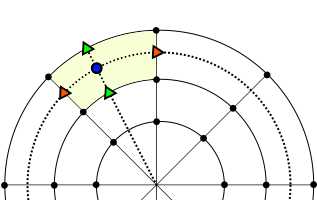
\includegraphics[width=\abImageWidth]{figures/spherical_interpolation.pdf}}
\caption{A 2-dimensional representation of the interpolation scheme that we employ on the spherical data. In the example we want to retrieve the value at the blue sampling location. While the (linear) radial interpolation provides the green values, the interpolation in $\phi$ produces the red values.}
\label{fig:sphericalvolume}
\end{figure}

\noindent {\bfseries Interpolation.} For each sample point along the ray, trilinear interpolation is performed along the $r$, $\phi$, and $\theta$ axes (see Figure~\ref{fig:sphericalvolume}). Using this scheme, the interpolation is effectively performed along great circles in the volume and thus performs analogous to Spherical Linear Interpolation (SLERP), creating a better interpolation result.

\noindent {\bfseries Adaptive sampling.} An additional aspect of the spherical volume to utilize is the sample distribution. While it is regular in spherical sample space, when converting samples into Cartesian world space, it is non-uniform with a density fall-off of $1/r^3$ (see Figure~\ref{fig:sphericalvolume}). It is possible to exploit the $1/r^3$ dependency in data density in the rendering step to perform data-aware importance sampling along the view ray. As the data density decreases in the outer areas of the sphere, it is sufficient to sample the view ray less dense. Likewise, it is beneficial to decrease the sampling step size closer to the origin. This technique is not limited to a spherical volume, but it is trivially integrated as the radial distance to the center is already available for each sample point. Using this technique, we achieved improved visual quality while, at the same time, increasing the rendering performance by 2$\times$.

\noindent {\bfseries Variables.} The ENLIL simulation code produces multi-variate datasets for each ensemble members. Of the 29 available variables for each simulation run, we utilize 4 in this part of our system. The $N \cdot r^2$ variable denotes the number of particles that are present in each voxel. The multiplication by $r^2$ negates the radial density falloff and allows us to utilize a single transfer function for the whole volume. The $\rho$ parameter is the density of particles. Together with the space weather analysts, we devised a method to make the simulation output more usable for volume rendering. Instead of running the simulation once, ENLIL now produces the CME-infused variables as before, but also produces a second set of variables only containing the solar wind, without the injected CME. For the purposes of the volume rendering, we display the difference between the two parameters $N \cdot r^2$ and $N \cdot r^2_\textrm{back}$. This results in a easier discrimination between the CME structure and the background wind, making the volume rendering easier to comprehend. We could perform the same operation for the velocity field as computed in Section~\ref{sec:simulationvelocity}, but the velocity of the background solar wind is 4-5 orders of magnitude lower than the speed of the CME. The $dp$ parameter is a set of tracer particles that are spawned in the cone denoting the CME. By advecting and tracing these particles between time steps, it is possible to use them as a segmentation mask for the CME. In order to perform the volume rendering, each sample point first samples the $dp$ volume which is used as a segmentation volume  -- modified by a transfer function --, and only samples the $N$ volume if the $dp$ transfer function response is positive.

\subsubsection{Integrated Rendering} \label{sec:integration}
In order to display the volume rendering combined with multiple geometries while allowing for transparency, we make use of an order-independent transparency method. Our system uses a per-fragment sorting technique that is based on an A-Buffer technique as presented by Lindholm~\etal~\cite{Lindholm:2014fm}. The technique operates by gathering fragments in a per-pixel linked list that is depth stored in a second pass, thus allowing for high-performant support of a sufficient level of depth complexity and the possibility of transparent objects integrated with volume rendering. 

\section{Application Case}
2014-04-18

The prediction error for the mean predicted CME arrival time was -5.2 hours and the observed arrival time was just within the ensemble predicted spread


\section{Future Work} \label{sec:futurework}
\begin{itemize}
\item 3D velocity reconstruction (inverse radon transform)
\item interpolating between satellites (cross-correlation)
\item include image-based techniques to select the CME for optical flow analysis
\item thompson scattering
\item image / optical flow filters specific for Cor2/HI1/HI2
\item provide an error metric to compare optical flow velocity fields and simulation velocity fields
\item use different fields to compare simulations and satellite images
\item interplanetary scintillation
\end{itemize}

%% if specified like this the section will be committed in review mode
\section*{Acknowledgments}
The presented visualization concepts have been realized using the Voreen framework (www.voreen.org). Simulation results have been provided by the Community Coordinated Modeling Center at Goddard Space Flight Center through their public Runs on Request system (http://ccmc.gsfc.nasa.gov). The CCMC is a multi-agency partnership between NASA, AFMC, AFOSR, AFRL, AFWA, NOAA, NSF and ONR.
%\nocite{*}


\bibliographystyle{abbrv}
%%use following if all content of bibtex file should be shown
%\nocite{*}
\bibliography{bibliography}
\end{document}

